\documentclass[10pt]{article}

\usepackage[utf8]{inputenc}
\usepackage[table,dvipsnames]{xcolor}
\usepackage{pdfpages} 
\usepackage[utf8]{inputenc}
\usepackage[english]{babel}
\usepackage{csquotes}
\usepackage{enumitem}
\usepackage{graphicx}
\usepackage{float}
\usepackage{fancyhdr}
\usepackage{longtable}
\usepackage{parskip}
\usepackage{amsmath}
\usepackage{svg}
% \usepackage{fontspec}

\usepackage[hidelinks]{hyperref}
\usepackage{cleveref}
\newcommand*{\fullref}[1]{\hyperref[{#1}]{\ref*{#1} \nameref*{#1}}}
\crefformat{footnote}{#2\footnotemark[#1]#3}

\usepackage{helvet}
\renewcommand{\familydefault}{\sfdefault}

\usepackage{todonotes}

% citations
\usepackage[style=ieee,backend=biber]{biblatex}
\usepackage[numberedsection]{glossaries-extra}
\addbibresource{./pa.bib}

% formatting
\topmargin -1cm 
\textheight 22cm
\textwidth 16.0 cm 
\oddsidemargin -0.1cm

\parindent=0pt
\setlength{\parskip}{12pt}
\linespread{1.2}

%table of content depth
\setcounter{tocdepth}{3}

\pagestyle{fancy}
\fancyhead[L]{\textbf{Project work} - Reviewing the state of the art in voice generation}
\fancyhead[R]{ZHAW - School of Engineering}

% handmade Keywords
\def\code#1{\texttt{#1}}
\patchcmd{\listoffigures}{\section*}{\section}{}{}
\patchcmd{\listoftables}{\section*}{\section}{}{}

\begin{document}
\begin{titlepage}
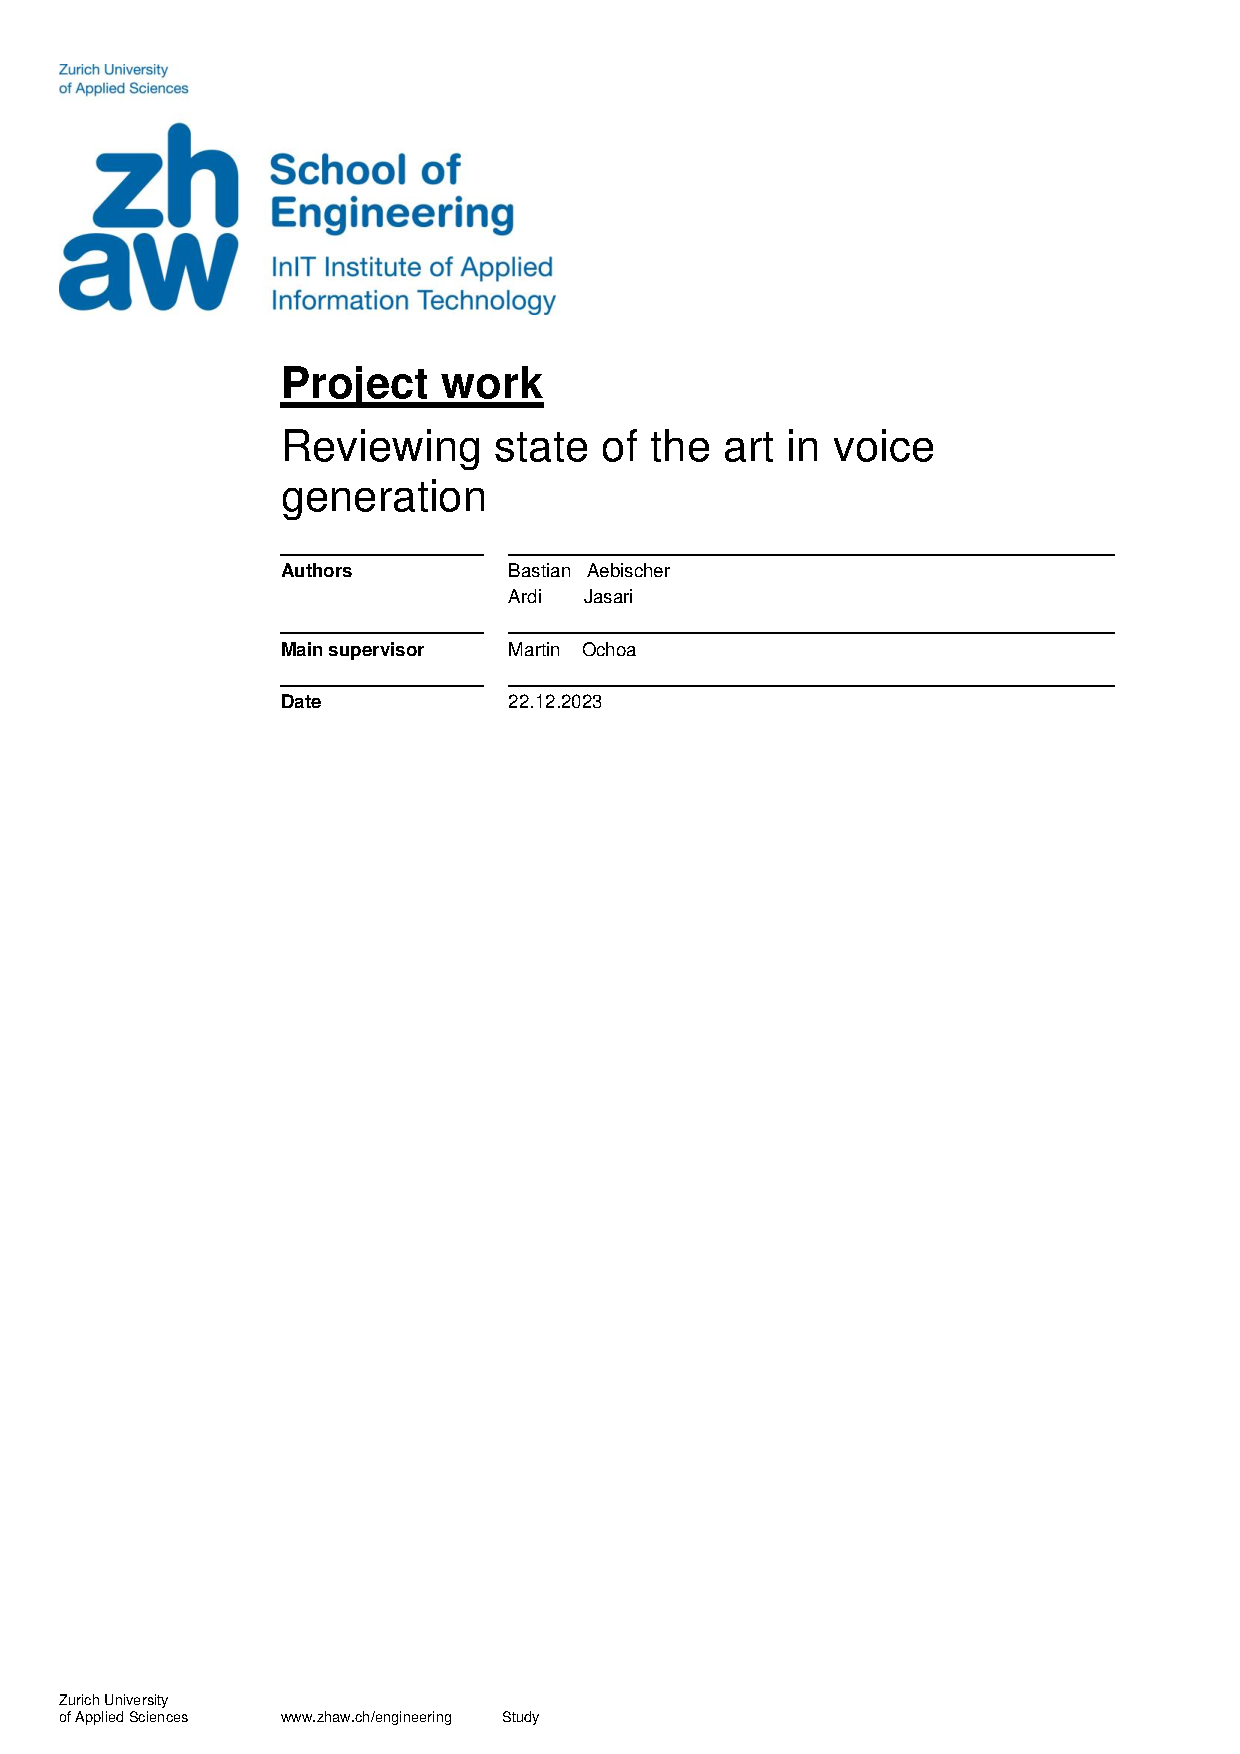
\includepdf[fitpaper=true, noautoscale=true, scale=0.9]{assets/pa_title.pdf}
\end{titlepage}

\pagenumbering{gobble}

\section*{Declaration of Originality}

\subsection*{Bachelor’s Thesis at the School of Engineering}

\paragraph{By submitting this Bachelor’s thesis, the undersigned student confirms that this thesis is his/her own work and was written without the help of a third party. (Group works: the performance of the other group members are not considered as third party).}

\paragraph{The student declares that all sources in the text (including Internet pages) and appendices have been correctly disclosed. This means that there has been no plagiarism, i.e. no sections of the Bachelor thesis have been partially or wholly taken from other texts and represented as the student’s own work or included without being correctly referenced.}

\paragraph{Any misconduct will be dealt with according to paragraphs 39 and 40 of the General Academic Regulations for Bachelor’s and Master’s Degree courses at the Zurich University of Applied Sciences (Rahmenprüfungsordnung ZHAW (RPO)) and subject to the provisions for disciplinary action stipulated in the University regulations.}

\begin{table}[b]
    \centering
    \begin{tabular}{ccc}
        \textbf{Place} &  \textbf{Date} & \textbf{Name} \\
        Winterthur & 22.12.2023 & \rule{5cm}{0.2mm} \\
        Winterthur & 22.12.2023 & \rule{5cm}{0.2mm} \\
    \end{tabular}
\end{table}

\thispagestyle{empty}
\input{chapters/00b_abstract}
\thispagestyle{empty}

\tableofcontents
\thispagestyle{empty}
\newpage

% chapters
\pagenumbering{arabic}

\newpage
\section{Introduction}

\subsection{Initial Situation}

Modern speech synthesis started in the 1960s, it began with huge databases of recorded speech that were cut into words and afterwards stitched back together during synthesizing. String of words were then reduced down to the individual diphones, which minimized the size of the databases significantly. In later years there was a statistical approach using a \gls{hmm}, where waveforms are formed based on probability. With the rapid expansion in the field of \gls{dnn} in the past years, voice generation based on \gls{ai} improved immensely as well.
These open-source implementations show great promise 
% TODO: short list of all technologies we want to introduce in chapter 2
.
Due to the big differences in implementations of speech synthesis and the subsequent voice conversion we focused on \gls{tts} synthesis and not on
% TODO: short list of disqualified technologies (singing voice synthesis, etc.)
.

More and more successful \gls{ai} voice scams have been reported % TODO: source needed
undeniably because of the increasingly realistic spoofed voice attacks. % real word?
Impersonation attacks over phone calls can become even easier and identity verification protocols based on voice id will soon be unfeasible. This puts great importance on raising awareness of the capabilities of such attacks and technologies to further improve possible detection or defense strategies and if these render futile, the deprecation of such security systems.


\subsection{Objective of this work}
The research question and objectives of this work are based on the official assignment on the subsection \ref{offassignment}.

The primary research question guiding this thesis is:
what is the current state of the art in voice generation, with a particular focus on the quality, ease of use, the potential limitations and risks of open source software implementations? 

To address the research question effectively, the following objectives have been defined:
\begin{itemize}
    \item Review state of the art for voice generation techniques:
    \begin{itemize}
        \item conduct an extensive search of literature on voice generation, focusing on recent developments in the field.
        \item Systematically classify identified voice generation techniques based on their underlying technologies. 
    \end{itemize}
    \item Select and evaluate most recent open source implementations:
    \begin{itemize}
        \item compare the different open source implementations subjectively and objectively through qualitative tests. 
        \item Compare the most recent software against an outdated solution highlighting improvements in recent implementations.
    \end{itemize}
    \item Analyze the potential limitations and risks:
    \begin{itemize}
        \item subjectively assess usability and ease of use, considering installation, intuitiveness of the user interface and accessibility of documentation.
        \item Examine robustness and stability of the implementations, by testing it under potential stress conditions, such as low-quality audio of the voice to be cloned.
        \item Test the synthesised voice on different voice authentication systems to assess its ability to pass authentication checks.
    \end{itemize}
\end{itemize}

\newpage
\section{Theoretical base}
This section is intended to describe the key components that usually compose a \gls{tts} system. This section does not go into the details of the individual components, but rather provides the basics for understanding the later sections. For more in-depth details, the references cited in this section can be consulted.

A \gls{tts} system normally consists of three components: a text analysis module, an acoustic model and a vocoder.

\subsection{Text Analysis Module}

The text analysis module processes the input text to extract linguistic features. Traditionally in \gls{spss} this process involved text processing, phonetic analysis and prosodic analysis\cite{Tan2023textanalysis}.

\textbf{Text processing:}
In this phase the document structure (e.g. headings, paragraphs) is analysed to apply appropriate prosody, rhythm, and intonation to the synthetised speech\cite{Tan2023textanalysis}. Subsequently, the non-standard words in the text (e.g. dates) are converted from written form into speakable form with text normalization\cite{Tan2023textanalysis, sproat2001normalization}. Linguistic analysis then extracts semantic information from the text\cite{Tan2023textanalysis}.

\textbf{Phonetic analysis:}
In phonetic analysis polyphone disambiguation is applied to distinguish the different pronunciations of the same word in different contexts. Furthermore, graphemes (sequence of characters) are converted into phonemes (sequence of pronunciation symbols), which facilitates speech synthesis\cite{Tan2023textanalysis, sun2019token}.

\textbf{Prosodic analysis:}
Prosodic analysis analyses the rhythm, stress, and intonation of speech. These features are important for achieving naturalness in synthesized speech\cite{Tan2023textanalysis}.

In neural \gls{tts} the text analysis module is often simplified, retaining only essential steps such as text normalization and grapheme-to-phoneme conversion. This approach enables the models to take phoneme sequences directly as input for the synthesis. This is driven by the capacity of neural networks to capture internal patterns and relationships directly from raw input data\cite{Tan2023textanalysis}.

\subsection{Acoustic Model}
Traditionally, in \gls{spss} the acoustic model takes the linguistic features as input to generate acoustic features, such as \gls{mcc}, \gls{bap}, and \gls{f0}, that represent the frequency components of the speech signal\cite{acoustic2023models, yoshimura1999simultaneous}. Techniques such as \gls{hmm} have been employed to generate these acoustic features\cite{tokuda2013speech}. Even though \gls{hmm}-based SPSS are more flexible in changing the voice characteristics compared to concatenative speech synthesis, the naturalness of synthesized speech is compromised due to the challenge of accurately modeling the complex acoustic features\cite{zen2015acoustic}.

In neural \gls{tts} systems acoustic models are enhanced with \gls{dnn}s. This eliminates the need for explicit alignments between linguistic and acoustic features, reducing preprocessing requirements. Furthermore, the representation of linguistic features simplifies to character or phoneme sequences, and acoustic features transition from low-dimensional representations to high-dimensional ones, such as mel-spectrograms or linear spectrograms\cite{acoustic2023models}.

Various model structures have been adopted in neural \gls{tts} acoustic models:

\textbf{RNN-Based Models (e.g., Tacotron series):} The Tacotron series leverages \gls{rnn}, employing an encoder-attention-decoder framework, to generate linear-scale spectrograms from character sequences\cite{wang2017tacotron, acoustic2023models}. Tacotron 2 uses the same acoustic model as in the original Tacotron to generate the mel-spectrograms. The main difference is in the vocoder utilized: Tacotron 2 utilizes a modified WaveNet vocoder, improving audio quality in comparison to the Griffin-Lim algorithm used in Tacotron\cite{shen2018natural}.

\textbf{CNN-Based Models (e.g., DeepVoice):} DeepVoice integrates \gls{cnn} into the \gls{spss} system, emphasizing the local dependencies of speech signals. Similarly to \gls{spss}, DeepVoice predicts the \gls{f0} for the entire duration of phonemes, with the major difference that it employs \gls{cnn}s to do so\cite{arik2017deep}.

\textbf{Transformer-Based Models (e.g., FastSpeech series):} %% explain also autoregressive transformer models because of tortoise 
The previous models, which all use autoregressive generation, have limitations such as slow inference and word skipping\cite{acoustic2023models}. the FastSpeech series introduces a feed-forward Transformer network that generates mel-spectrograms in parallel, speeding up training and inference, and improving robustness\cite{ren2019fastspeech, ren2021fastspeech}.

\textbf{Advanced Generative Models (GAN/Flow/VAE/Diffusion):} To handle the distributional nature of mel-spectrogram data conditioned on phoneme sequences, advanced generative models, such as \gls{gan}, normalizing flow, \gls{vae}, and diffusion model, are introduced. These models contribute to generating high-quality mel-spectrograms with fine-grained details.

Diffusion models in \gls{tts} operate on the principle of enhancing the quality of the mel-spectrograms by iteratively removing noise. This denoising process necessitates a large number of iteration steps considerably slowing down inference speed\cite{acoustic2023models}.

\subsection{Vocoder}

The vocoder is the part of voice generation that takes the context from the outputs of text analysis modules and or from acoustic models, and synthesizes the actual audio, meaning waveforms that can be listened to on their preferred medium. In the focus of digital voice generation one does generally differentiate between vocoders from a signal-processing-based approach and vocoders from a neural-network-based approach\cite{Tan2023vocoder}.

We take a look at different neural-network based vocoders that are used in the systems we considered.

\subsubsection{UnivNet}

UnivNet is a neural vocoder developed in South Korea that synthesizes high-fidelity waveforms in real time. Instead of only using band-limitied mel-spectograms, which can produce over-smoothing problems; UnivNet accepts multiple spectograms generated or real then applies a multi-resolution spectrogram discriminator. The main difference lies in the spectrograms used in UnivNet are chosen based on different spectral and temporal resolutions. Finally there is also a multi-period waveform discriminator\cite{jang2021univnet}.

\subsubsection{WaveNet}

WaveNet is a deep neural network developed by Google. It is an audio generative model based on the PixelCNN architecture that is fully probabilistic and autoregressive. WaveNet combines causal filters with dilated convolutions to allow their receptive fields to grow exponentially with depth, which is important to model
the long-range temporal dependencies in audio signals\cite{oord2016wavenet}.

\subsection{Fully End-to-End TTS}

Figure \ref{fig:end-to-end} shows an overview of the different modules voice generation systems can be composed and also which parts do the similar work. Even though the inputs are not the same for each process the overarching theme is still generally the same. Namely it starts from thought concepts that are written down and try to communicate a meaning within their context of application and it ends with the synthesizing of binary data to the finalized waveforms.
Now comes the last process which incorporates all different modules into one model : a fully end-to-end \gls{tts} model.

An end-to-end system tries to optimize the different shortcomings of marrying multiple single components into one system. These are:
\begin{itemize}
    \item Reducing human supervision of the feature alignments,
    \item Optimising of error propagation in cascaded models,
    \item Saving time and resources during training and deployment.
\end{itemize}
\cite{Tan2023fullyendtoend}

 \begin{figure}[H]
    \centering
    \includegraphics[width=1\linewidth]{assets/end-to-end.PNG}
    \caption{The progressively end-to-end process for TTS models\cite{Tan2023fullyendtoend}}
    \label{fig:end-to-end}
\end{figure}


\newpage
\section{Methods} \label{methods}

In this section we describe our methods that we used to make a preselection of different voice generation solutions and then the process where we refined the preselection.
It first started with the introduction text from our project work description. In the description the key words are generative AI, voice generation / voice synthesis, open source implementations and machine learning / deep neural networks. Additionally there is also new report linked from CBS News \cite{cbsnews2023voice}, where CBS reports an uptick in elevated scams using cloned speech and also describes how with the new tools like Vall-E a scammer only needs 3 seconds of the targets voice to create a copy that can then be used against potential victims.

\subsection{Academic Research}

With the guidance of our supervisor we started with multiple surveys in scientific papers and followed all the trails that promised us new knowledge. The most helpful were "Spoofing and countermeasures for speaker verification: A survey" by Zhizheng Wu et al.\cite{wu2015spoofing} and "A survey on voice assistant security: Attacks and countermeasures" by Chen Yan et al.\cite{yan2022survey}.

There are three main approaches for AI voice imitation: Voice conversion models that need an audio sample from the target voice(the voice to be imitated) and an audio recording of the target speech(the sentences to be imitated), singing voice synthesis that work similar to a voice conversion model but are more finetuned for intonation used when singing and last but not least there is the \gls{tts} synthesis that needs a target voice sample and the target speech in text format.

\todo[inline]{add more interesting papers}

\subsection{Github}

As one focus of this paper is to find out how easy it would be for an attacker to fake the voice of a potential victim, we concentrate on open source implementations. These are commonly found on \url{https://www.github.com}. First method was searching for keywords via a search engine, some of the keywords were: "AI voice generation", "voice synthesis", "text-to-speech", "voice conversion", etc.. Finding interesting repositories it is then to evaluate them based on objective criteria. For us these criteria were:
\begin{itemize}
    \item \textbf{Actively maintained:} When was the latest feature merge? Is the project still in development or is it finished? How is the activity on open issues?
    \item \textbf{Amount of stars:} Staring is the github equivalent to liking or giving a thumbs up. It is a way of adding a \gls{repo} to the users list or for showing their appreciation. Generally the more popular a \gls{repo} is the more stars it has.
    \item \textbf{Amount of forks:} This metric can be similar to the amount of stars, but it also shows how a \gls{repo}s is established as a solution that it is trying to solve. The more forks a project has, the more it can be looked at as a standard for this specific solution.
    \item \textbf{Available training data:} Is the training data integrated in the \gls{repo}? Are there links to tried and tested training data? Or is one expected to train the model by themselves?
    \item \textbf{Available languages:} Does it only support English? Does it only support Chinese? Does \gls{repo} support a wide range of languages?
    \item \textbf{Implementations of papers:} Are there any papers referenced in the \gls{repo}?
    \item \textbf{Possible affiliation with companies/governments:} Is \gls{repo} linked to a paper that was published with the special funding of companies or governments? Is it part of a business solution that a company is offering for money?
\end{itemize}

After finding good candidates most often the \gls{repo} are well maintained and with that they ususally are correctly categorized into the appropriate topics. The connected topics are thereupon a great follow-up, if the \gls{repo} was not good enough but the topic shows promise. We identified the following topics: "spech", "text-to-speech", "deep-learning", "speech-synthesis", "voice-synthesis", "melgan", "multi-speaker-tts", "voice-cloning", "tacotron" and "vocoder".

\subsection{Output Evaluation}

\todo[inline]{General description, general comments(quality, duration, frequent/emerging patterns, settings used), Picture-comparison, conclusion about best sample}

% explain why we used pangrams and explain each sentence

%to select the open source implementations we looked at the following things: start on the github reposisory. Is there a pretrained model? Can we clone own voice? Is it still maintaned (date of last commit)? Is it new? Zero shot TTS

% which sentences we used to test the open-source implementations? what metrics did we use to evaluate the results (Mean Opinion Score)? (5:Excellent, 4:Good, 3:Fair, 2:Poor, 1:Bad)


\newpage
\section{Results}

Ut molestiae nesciunt tenetur. Veritatis odio aliquid omnis porro neque et. Sit autem dolorum blanditiis aut cupiditate qui.
Voluptate in dolore error consequatur rerum enim velit. Magnam tenetur sunt voluptatem et placeat rerum. Ea error repellat doloribus rerum qui sapiente numquam. Culpa laboriosam quia illum iure sit pariatur eum. Quos qui animi occaecati nesciunt repellendus molestiae commodi. Dolor nam ullam debitis dolorem quam.
\newpage
\section{Discussion}

The evaluation of speech is subjective due to the complexity of human perception. The influence of training data and inference iterations on the quality of speech synthesis is a crucial aspect to consider. This can be observed with TorToise, which demonstrated remarkable naturalness in its synthesized output, attributed to the extensive training data set and a high number of inference iterations. However, the speaker similarity aspect did not exhibit a proportional improvement, as evidenced by the comparable speaker similarity results observed in TorToise, trained on a significantly larger data set, and VALL-E X, trained on a comparatively smaller data set. The nature of the training data further influences the output characteristics, evident in TorToise's distinctive book reading style, a reflection of its primary training on audio books.

The candidate generation played a significant role in obtaining natural synthesized speech. TorToise seamlessly handled this step through the Contrastive Language-Voice Pretrained Transformer (CLVP), automating the generation and selection of optimal speech tokens. Additionally three output candidates were generated and the best one was manually selected. In contrast, VALL-E X required manual generation of multiple candidates by synthesizing the same sentence repeatedly. Multiple candidates were needed especially for sentences featuring complex phonemes and uncommon words in VALL-E X, highlighting potential limitations in the diversity of its training data concerning these linguistic elements.
The quantity of training data alone does not guarantee success, as observed in Real-Time Voice Cloning. Despite being trained on a larger dataset compared to VALL-E X, Real-Time Voice Cloning, being an earlier tool, did not generate natural sounding speech. This underscores the importance of recent advancements in model architectures in \gls{dnn}.

%own mistakes?

The results from this research shows the current capabilities of \gls{dnn}s synthesizing speech and how the quality can be, when generating speech for potential scams or spoofing attacks. Most of the generated audio is not usable in voice spoofing attacks due to clearly being recognized as generated speech with robotic-sounding artefacts, wrong intonations or bad-sounding prosody. These negative properties can be diminished when using them in situations, where worse audio quality is a plausibility. For example phone calls with bad audio quality either due to a bad microphone or bad reception while going through tunnels or calling from remote areas with less signal. With modern voice-over-internet-protocol calls the quality is usually good enough to notice synthesized speech. Considering the long generation times the need of a pre-generated response set is mandatory for a spoofing attack over a phone call. Additionally this means generating a lot of different responses to accommodate many situations in a phone call. A more ideal situation for an attacker is the use of voice messages, so sending recorded speech in replacement of a phone call. There, an attacker has much more time to generate the best possible response while also having the option to generate speech displaying emotions. Though with voice messages one does need to have access to a verified device from the targeted person to properly impersonate them. Sending voice messages with synthesized speech can be interpreted as more plausible as just plain text, when having access to a verified device through theft or spoofing. The best defense against these attacks is to ask the possible attacker on the phone for a completely random passphrase from a shared experience between them or a more elaborate system ask them for an explanation of a word from the dictionary the longer the explanation the better the system. For example: "Can you please explain to me what a guitar is?".

All these reasons naturally change when one tries to imitate a well-known person with a lot of recorded material readily available, for example celebrities, politicians, CEOs or people in general working in front of a camera or microphone such as actors, news anchors, journalists, podcast hosts et cetera. With extensive audio material one can even train \gls{dnn}s on these persons to achieve even more convincing synthesized speech from these models. If one abstracts this imitation problem to the extreme, it condenses into a probabilistic problem where each audio file is a sequence of binary data that translated into sound waves could be unrecognizable to the binary sequence of a recording of a real person. Obviously with so many variables it will take a lot of time to produce such results, but at a certain point the fake voice sounds exactly the same as the real voice to a loudspeaker. Such problems can most often only be solved by cryptography, meaning in the future where such perfect imitations are possible, the best way to verify the authenticity of any voice transmission will be a Diffie-Hellman key exchange with verified sources\cite{maurer2000diffie}.

\clearpage

\nocite{*}
\printbibliography[heading=bibnumbered]

%\listoffigures
%\listoftables
%\clearpage

\end{document}
